% !TEX root = ../main.tex
% !TEX program = xelatex

\chapter{ExRORU算法的唯一性补充说明}
\label{app:uniqueness}
对过程模型$P$结构上的任意单步变动产生了新的过程模型$Q$,可以从三个方面证明$P$和$Q$的ExRORU矩阵是不同的:(1)改变一对变迁间的关系;(2)增加/删除一个可见变迁;(3)增加/删除一个不可见变迁。接下来用图示法从三个方面分别说明。

{\heiti(1)改变一对变迁间的关系:}如果一对关系被改变了,例如一对处于顺序结构中的变迁被改造成并行结构或者循环结构,这类基本关系的改变显然会直接反映在模型的ExRORU矩阵中,在此不加赘述。

{\heiti(2)增加/删除一个可见变迁:}一个新的可见变迁可以被添加在过程模型中,且其必然会与一个已有的变迁(更一般化地,与一个包含多个变迁和库所的子过程)同处一个顺序结构、或并行结构、或互斥结构、或循环结构,如图\ref{fig:uniqueness_2}所示。为便于展示,图中只展示了一个WF-net的部分结构,$A$和$B$是两个不同的变迁,带斜线的阴影框表示不可见变迁。矩阵中的$A$和$B$对应图中的两个变迁,$S$代表该部分结构前与之紧邻的前驱变迁,$E$代表该部分结构后与之紧邻的后继变迁。
\begin{enumerate}[(a)]
  \item 原始模型的部分结构,只含有一个可见变迁$A$,如图\ref{fig:uniqueness_2_a}。
  \item 在变迁$A$之后增加一个可见变迁$B$,与变迁$A$同处顺序结构,如图\ref{fig:uniqueness_2_b}。此时ExRORU矩阵多了有关变迁$B$的行列,显然发生了改变。
  \item 在变迁$A$之前增加一个可见变迁$B$,与变迁$A$同处顺序结构,如图\ref{fig:uniqueness_2_c}。此时ExRORU矩阵多了有关变迁$B$的行列,显然发生了改变。
  \item 增加一个可见变迁$B$,与$A$同处互斥结构,如图\ref{fig:uniqueness_2_d}。此时ExRORU矩阵多了有关变迁$B$的行列,显然发生了改变。而且,变迁$S$与变迁$A$的因果关系从“直接总是因果关系”变为“直接有时因果关系”,即$S\overset{\text{\tiny{DA}}}{\rightarrow}A\Rightarrow S\overset{\text{\tiny{DS}}}{\rightarrow}A$;变迁$E$与变迁$A$的逆因果关系从“直接总是逆因果关系”变为“直接有时逆因果关系”,即$E\overset{\text{\tiny{DA}}}{\leftarrow}A\Rightarrow E\overset{\text{\tiny{DS}}}{\leftarrow}A$。
  \item 增加一个可见变迁$B$,与$A$同处循环结构,如图\ref{fig:uniqueness_2_e}。此时ExRORU矩阵多了有关变迁$B$的行列,显然发生了改变。而且,变迁$A$与变迁$S$的逆因果关系从“直接总是逆因果关系”变为“直接有时逆因果关系”,即$A\overset{\text{\tiny{DA}}}{\leftarrow}S\Rightarrow A\overset{\text{\tiny{DS}}}{\leftarrow}S$;变迁$A$与变迁$E$的因果关系从“直接总是因果关系”变为“直接有时因果关系”,即$A\overset{\text{\tiny{DA}}}{\rightarrow}E\Rightarrow A\overset{\text{\tiny{DS}}}{\rightarrow}E$;变迁$A$与其自身的因果关系和逆因果关系从“从不因果关系”和“从不逆因果关系”变为“间接有时因果关系”和“间接有时逆因果关系”,即$A\overset{\text{\tiny{N}}}{\rightarrow}A,A\overset{\text{\tiny{N}}}{\leftarrow}A\Rightarrow A\overset{\text{\tiny{IS}}}{\rightarrow}A,A\overset{\text{\tiny{IS}}}{\leftarrow}A$。
  \item 增加一个可见变迁$B$,与$A$同处并行结构,如图\ref{fig:uniqueness_2_f}。此时ExRORU矩阵多了有关变迁$B$的行列,显然发生了改变。
\end{enumerate}
从图中可以看出,上述所有变化都会导致对应的ExRORU矩阵发生变化。因为一个新的过程模型是通过将上述单步变化连续应用在原始过程模型中产生的,归纳可知新的过程模型和原始模型拥有不同的ExRORU矩阵。类似的证明可应用于“删除一个可见变迁”中。

{\heiti(3)增加/删除一个不可见变迁:}一个新的不可见变迁也可以被添加在过程模型中,与情形(2)中的结构类似,如图\ref{fig:uniqueness_3}所示。
\begin{enumerate}[(a)]
  \item 原始模型的部分结构,只含有一个可见变迁$A$,如图\ref{fig:uniqueness_3_a}。
  \item 将变迁$A$两侧的库所合并成一个库所,如图\ref{fig:uniqueness_3_b}。变迁$S$和变迁$A$的因果关系、变迁$A$和变迁$S$的逆因果关系从“直接总是因果关系”、“直接总是逆因果关系”变为“直接有时因果关系”、“直接有时逆因果关系”,即$S\overset{\text{\tiny{DA}}}{\rightarrow}A,A\overset{\text{\tiny{DA}}}{\leftarrow}S\Rightarrow S\overset{\text{\tiny{DS}}}{\rightarrow}A,A\overset{\text{\tiny{DS}}}{\leftarrow}S$;变迁$A$和变迁$E$的因果关系、变迁$E$和变迁$A$的逆因果关系从“直接总是因果关系”、“直接总是逆因果关系”变为“直接有时因果关系”、“直接有时逆因果关系”,即$A\overset{\text{\tiny{DA}}}{\rightarrow}E,E\overset{\text{\tiny{DA}}}{\leftarrow}A\Rightarrow A\overset{\text{\tiny{DS}}}{\rightarrow}E,E\overset{\text{\tiny{DS}}}{\leftarrow}A$;变迁$A$与其自身的因果关系和逆因果关系从“从不因果关系”和“从不逆因果关系”变为“直接有时因果关系”和“直接有时逆因果关系”,即$A\overset{\text{\tiny{N}}}{\rightarrow}A,A\overset{\text{\tiny{N}}}{\leftarrow}A\Rightarrow A\overset{\text{\tiny{DS}}}{\rightarrow}A,A\overset{\text{\tiny{DS}}}{\leftarrow}A$;变迁$S$和变迁$E$的因果关系、变迁$E$与变迁$S$的逆因果关系从“间接总是因果关系”、“间接总是逆因果关系”变为“直接总是因果关系”、“直接总是逆因果关系”,即$S\overset{\text{\tiny{IA}}}{\rightarrow}E,E\overset{\text{\tiny{IA}}}{\leftarrow}S\Rightarrow S\overset{\text{\tiny{DA}}}{\rightarrow}E,E\overset{\text{\tiny{DA}}}{\leftarrow}S$。
  \item 增加一个不可见变迁,与$A$同处互斥结构,如图\ref{fig:uniqueness_3_c}。变迁$S$与变迁$A$的因果关系从“直接总是因果关系”变为“直接有时因果关系”,即$S\overset{\text{\tiny{DA}}}{\rightarrow}A\Rightarrow S\overset{\text{\tiny{DS}}}{\rightarrow}A$;变迁$E$与变迁$A$的逆因果关系从“直接总是逆因果关系”变为“直接有时逆因果关系”,即$E\overset{\text{\tiny{DA}}}{\leftarrow}A\Rightarrow E\overset{\text{\tiny{DS}}}{\leftarrow}A$;变迁$S$和变迁$E$的因果关系、变迁$E$与变迁$S$的逆因果关系从“间接总是因果关系”、“间接总是逆因果关系”变为“直接总是因果关系”、“直接总是逆因果关系”,即$S\overset{\text{\tiny{IA}}}{\rightarrow}E,E\overset{\text{\tiny{IA}}}{\leftarrow}S\Rightarrow S\overset{\text{\tiny{DA}}}{\rightarrow}E,E\overset{\text{\tiny{DA}}}{\leftarrow}S$。
  \item 增加一个不可见变迁,与$A$同处循环结构,如图\ref{fig:uniqueness_3_d}。变迁$A$和变迁$S$的逆因果关系从“直接总是逆因果关系”变为“直接有时逆因果关系”,即$A\overset{\text{\tiny{DA}}}{\leftarrow}S\Rightarrow A\overset{\text{\tiny{DS}}}{\leftarrow}S$;变迁$A$和变迁$E$的因果关系从“直接总是因果关系”变为“直接有时因果关系”,即$A\overset{\text{\tiny{DA}}}{\rightarrow}E\Rightarrow A\overset{\text{\tiny{DS}}}{\rightarrow}E$;变迁$A$与其自身的因果关系和逆因果关系从“从不因果关系”和“从不逆因果关系”变为“直接有时因果关系”和“直接有时逆因果关系”,即$A\overset{\text{\tiny{N}}}{\rightarrow}A,A\overset{\text{\tiny{N}}}{\leftarrow}A\Rightarrow A\overset{\text{\tiny{DS}}}{\rightarrow}A,A\overset{\text{\tiny{DS}}}{\leftarrow}A$。
  \item 另一个原始模型的部分结构,含有两个处于并行结构的变迁$A$和变迁$B$,如图\ref{fig:uniqueness_3_e}。
  \item 增加一个不可见变迁,与$B$同处互斥结构,如图\ref{fig:uniqueness_3_f}。变迁$S$和变迁$B$的因果关系从“直接总是因果关系”变为“直接有时因果关系”,即$S\overset{\text{\tiny{DA}}}{\rightarrow}B\Rightarrow S\overset{\text{\tiny{DS}}}{\rightarrow}B$;变迁$E$和变迁$B$的逆因果关系从“直接总是逆因果关系”变为“直接有时逆因果关系”,即$E\overset{\text{\tiny{DA}}}{\leftarrow}B\Rightarrow E\overset{\text{\tiny{DS}}}{\leftarrow}B$;变迁$A$和变迁$B$的并行关系从“总是并行关系”变为“有时并行关系”,即$A\Updownarrow B\Rightarrow A\Uparrow B$。
  \item 增加一个不可见变迁,与$A$同处互斥结构,如图\ref{fig:uniqueness_3_g}。变迁$S$和变迁$A$的因果关系从“直接总是因果关系”变为“直接有时因果关系”,即$S\overset{\text{\tiny{DA}}}{\rightarrow}A\Rightarrow S\overset{\text{\tiny{DS}}}{\rightarrow}A$;变迁$E$和变迁$A$的逆因果关系从“直接总是逆因果关系”变为“直接有时逆因果关系”,即$E\overset{\text{\tiny{DA}}}{\leftarrow}A\Rightarrow E\overset{\text{\tiny{DS}}}{\leftarrow}A$;变迁$B$和变迁$A$的并行关系从“总是并行关系”变为“有时并行关系”,即$B\Updownarrow A\Rightarrow B\Uparrow A$。
  \item 增加一个不可见变迁,与$B$同处循环结构,如图\ref{fig:uniqueness_3_h}。变迁$B$和变迁$S$的逆因果关系从“直接总是逆因果关系”变为“直接有时逆因果关系”,即$B\overset{\text{\tiny{DA}}}{\leftarrow}S\Rightarrow B\overset{\text{\tiny{DS}}}{\leftarrow}S$;变迁$B$和变迁$E$的因果关系从“直接总是因果关系”变为“直接有时因果关系”,即$B\overset{\text{\tiny{DA}}}{\rightarrow}E\Rightarrow B\overset{\text{\tiny{DS}}}{\rightarrow}E$;变迁$B$与其自身的因果关系和逆因果关系从“从不因果关系”和“从不逆因果关系”变为“直接有时因果关系”和“直接有时逆因果关系”,即$B\overset{\text{\tiny{N}}}{\rightarrow}B,B\overset{\text{\tiny{N}}}{\leftarrow}B\Rightarrow B\overset{\text{\tiny{DS}}}{\rightarrow}B,B\overset{\text{\tiny{DS}}}{\leftarrow}B$;变迁$B$和变迁$A$的并行关系从“总是并行关系”变为“有时并行关系”,即$B\Updownarrow A\Rightarrow B\Uparrow A$。
  \item 增加一个不可见变迁,与$A$同处循环结构,如图\ref{fig:uniqueness_3_i}。变迁$A$和变迁$S$的逆因果关系从“直接总是逆因果关系”变为“直接有时逆因果关系”,即$A\overset{\text{\tiny{DA}}}{\leftarrow}S\Rightarrow A\overset{\text{\tiny{DS}}}{\leftarrow}S$;变迁$A$和变迁$E$的因果关系从“直接总是因果关系”变为“直接有时因果关系”,即$A\overset{\text{\tiny{DA}}}{\rightarrow}E\Rightarrow A\overset{\text{\tiny{DS}}}{\rightarrow}E$;变迁$A$与其自身的因果关系和逆因果关系从“从不因果关系”和“从不逆因果关系”变为“直接有时因果关系”和“直接有时逆因果关系”,即$A\overset{\text{\tiny{N}}}{\rightarrow}A,A\overset{\text{\tiny{N}}}{\leftarrow}A\Rightarrow A\overset{\text{\tiny{DS}}}{\rightarrow}A,A\overset{\text{\tiny{DS}}}{\leftarrow}A$;变迁$A$和变迁$B$的并行关系从“总是并行关系”变为“有时并行关系”,即$A\Updownarrow B\Rightarrow A\Uparrow B$。
\end{enumerate}
任意单步变化都会导致对应的ExRORU矩阵发生变化,根据归纳法可知将上述单步变化连续应用在原始过程模型中产生的新过程模型拥有与原始模型不同的ExRORU矩阵。类似的证明可应用于“删除一个不可见变迁”中。

\begin{figure}[htbp]
  \centering

  \begin{subfigure}{1\textwidth}
    \centering
    \begin{minipage}[b]{1\textwidth}
      \centering
      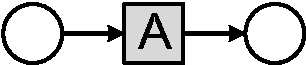
\includegraphics[width=0.3\textwidth]{uniqueness_2_a}
    \end{minipage}
    \begin{minipage}[b]{0.3\textwidth}
      \vspace{1em}
      \centering
      \begin{tabular}{|c|c|c|c|} \hline
        $\rightarrow$ & $\bm{S}$ & $A$ & $\bm{E}$\\ \hline
        $\bm{S}$ & $\overset{\text{\tiny{N}}}{\rightarrow}$ & $\overset{\text{\tiny{DA}}}{\rightarrow}$ & $\overset{\text{\tiny{IA}}}{\rightarrow}$\\ \hline
        $A$ & $\overset{\text{\tiny{N}}}{\rightarrow}$ & $\overset{\text{\tiny{N}}}{\rightarrow}$ & $\overset{\text{\tiny{DA}}}{\rightarrow}$\\ \hline
        $\bm{E}$ & $\overset{\text{\tiny{N}}}{\rightarrow}$ & $\overset{\text{\tiny{N}}}{\rightarrow}$ & $\overset{\text{\tiny{N}}}{\rightarrow}$\\ \hline
      \end{tabular}
    \end{minipage}
    \begin{minipage}[b]{0.3\textwidth}
      \vspace{1em}
      \centering
      \begin{tabular}{|c|c|c|c|} \hline
        $\leftarrow$ & $\bm{S}$ & $A$ & $\bm{E}$\\ \hline
        $\bm{S}$ & $\overset{\text{\tiny{N}}}{\leftarrow}$ & $\overset{\text{\tiny{N}}}{\leftarrow}$ & $\overset{\text{\tiny{N}}}{\leftarrow}$\\ \hline
        $A$ & $\overset{\text{\tiny{DA}}}{\leftarrow}$ & $\overset{\text{\tiny{N}}}{\leftarrow}$ & $\overset{\text{\tiny{N}}}{\leftarrow}$\\ \hline
        $\bm{E}$ & $\overset{\text{\tiny{IA}}}{\leftarrow}$ & $\overset{\text{\tiny{DA}}}{\leftarrow}$ & $\overset{\text{\tiny{N}}}{\leftarrow}$\\ \hline
      \end{tabular}
    \end{minipage}
    \begin{minipage}[b]{0.3\textwidth}
      \vspace{1em}
      \centering
      \begin{tabular}{|c|c|c|c|} \hline
        $\parallel$ & $\bm{S}$ & $A$ & $\bm{E}$\\ \hline
        $\bm{S}$ & $\nparallel$ & $\nparallel$ & $\nparallel$\\ \hline
        $A$ & $\nparallel$ & $\nparallel$ & $\nparallel$\\ \hline
        $\bm{E}$ & $\nparallel$ & $\nparallel$ & $\nparallel$\\ \hline
      \end{tabular}
    \end{minipage}
    \caption{原始部分模型,只含有可见变迁$A$}
    \label{fig:uniqueness_2_a}
  \end{subfigure}

  \begin{subfigure}{1\textwidth}
    \vspace{1em}
    \centering
    \begin{minipage}[b]{1\textwidth}
      \centering
      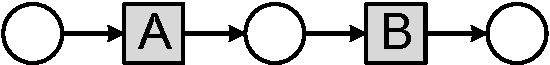
\includegraphics[width=0.5\textwidth]{uniqueness_2_b}
    \end{minipage}
    \begin{minipage}[b]{0.3\textwidth}
      \vspace{1em}
      \centering
      \begin{tabular}{|c|c|c|c|c|} \hline
        $\rightarrow$ & $\bm{S}$ & $A$ & $B$ & $\bm{E}$\\ \hline
        $\bm{S}$ & $\overset{\text{\tiny{N}}}{\rightarrow}$ & $\overset{\text{\tiny{DA}}}{\rightarrow}$ & $\overset{\text{\tiny{IA}}}{\rightarrow}$ & $\overset{\text{\tiny{IA}}}{\rightarrow}$\\ \hline
        $A$ & $\overset{\text{\tiny{N}}}{\rightarrow}$ & $\overset{\text{\tiny{N}}}{\rightarrow}$ & $\overset{\text{\tiny{DA}}}{\rightarrow}$ & $\overset{\text{\tiny{IA}}}{\rightarrow}$\\ \hline
        $B$ & $\overset{\text{\tiny{N}}}{\rightarrow}$ & $\overset{\text{\tiny{N}}}{\rightarrow}$ & $\overset{\text{\tiny{N}}}{\rightarrow}$ & $\overset{\text{\tiny{DA}}}{\rightarrow}$\\ \hline
        $\bm{E}$ & $\overset{\text{\tiny{N}}}{\rightarrow}$ & $\overset{\text{\tiny{N}}}{\rightarrow}$ & $\overset{\text{\tiny{N}}}{\rightarrow}$ & $\overset{\text{\tiny{N}}}{\rightarrow}$\\ \hline
      \end{tabular}
    \end{minipage}
    \begin{minipage}[b]{0.3\textwidth}
      \vspace{1em}
      \centering
      \begin{tabular}{|c|c|c|c|c|} \hline
        $\leftarrow$ & $\bm{S}$ & $A$ & $B$ & $\bm{E}$\\ \hline
        $\bm{S}$ & $\overset{\text{\tiny{N}}}{\leftarrow}$ & $\overset{\text{\tiny{N}}}{\leftarrow}$ & $\overset{\text{\tiny{N}}}{\leftarrow}$ & $\overset{\text{\tiny{N}}}{\leftarrow}$\\ \hline
        $A$ & $\overset{\text{\tiny{DA}}}{\leftarrow}$ & $\overset{\text{\tiny{N}}}{\leftarrow}$ & $\overset{\text{\tiny{N}}}{\leftarrow}$ & $\overset{\text{\tiny{N}}}{\leftarrow}$\\ \hline
        $B$ & $\overset{\text{\tiny{IA}}}{\leftarrow}$ & $\overset{\text{\tiny{DA}}}{\leftarrow}$ & $\overset{\text{\tiny{N}}}{\leftarrow}$ & $\overset{\text{\tiny{N}}}{\leftarrow}$\\ \hline
        $\bm{E}$ & $\overset{\text{\tiny{IA}}}{\leftarrow}$ & $\overset{\text{\tiny{IA}}}{\leftarrow}$ & $\overset{\text{\tiny{DA}}}{\leftarrow}$ & $\overset{\text{\tiny{N}}}{\leftarrow}$\\ \hline
      \end{tabular}
    \end{minipage}
    \begin{minipage}[b]{0.3\textwidth}
      \vspace{1em}
      \centering
      \begin{tabular}{|c|c|c|c|c|} \hline
        $\parallel$ & $\bm{S}$ & $A$ & $B$ & $\bm{E}$\\ \hline
        $\bm{S}$ & $\nparallel$ & $\nparallel$ & $\nparallel$ & $\nparallel$\\ \hline
        $A$ & $\nparallel$ & $\nparallel$ & $\nparallel$ & $\nparallel$\\ \hline
        $B$ & $\nparallel$ & $\nparallel$ & $\nparallel$ & $\nparallel$\\ \hline
        $\bm{E}$ & $\nparallel$ & $\nparallel$ & $\nparallel$ & $\nparallel$\\ \hline
      \end{tabular}
    \end{minipage}
    \caption{在\subref{fig:uniqueness_2_a}中的变迁$A$之后增加一个可见变迁$B$,与$A$同处顺序结构}
    \label{fig:uniqueness_2_b}
  \end{subfigure}

  \begin{subfigure}{1\textwidth}
    \vspace{1em}
    \centering
    \begin{minipage}[b]{1\textwidth}
      \centering
      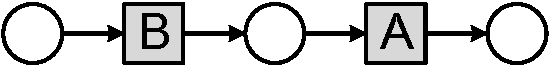
\includegraphics[width=0.5\textwidth]{uniqueness_2_c}
    \end{minipage}
    \begin{minipage}[b]{0.3\textwidth}
      \vspace{1em}
      \centering
      \begin{tabular}{|c|c|c|c|c|} \hline
        $\rightarrow$ & $\bm{S}$ & $A$ & $B$ & $\bm{E}$\\ \hline
        $\bm{S}$ & $\overset{\text{\tiny{N}}}{\rightarrow}$ & $\overset{\text{\tiny{IA}}}{\rightarrow}$ & $\overset{\text{\tiny{DA}}}{\rightarrow}$ & $\overset{\text{\tiny{IA}}}{\rightarrow}$\\ \hline
        $A$ & $\overset{\text{\tiny{N}}}{\rightarrow}$ & $\overset{\text{\tiny{N}}}{\rightarrow}$ & $\overset{\text{\tiny{N}}}{\rightarrow}$ & $\overset{\text{\tiny{DA}}}{\rightarrow}$\\ \hline
        $B$ & $\overset{\text{\tiny{N}}}{\rightarrow}$ & $\overset{\text{\tiny{DA}}}{\rightarrow}$ & $\overset{\text{\tiny{N}}}{\rightarrow}$ & $\overset{\text{\tiny{IA}}}{\rightarrow}$\\ \hline
        $\bm{E}$ & $\overset{\text{\tiny{N}}}{\rightarrow}$ & $\overset{\text{\tiny{N}}}{\rightarrow}$ & $\overset{\text{\tiny{N}}}{\rightarrow}$ & $\overset{\text{\tiny{N}}}{\rightarrow}$\\ \hline
      \end{tabular}
    \end{minipage}
    \begin{minipage}[b]{0.3\textwidth}
      \vspace{1em}
      \centering
      \begin{tabular}{|c|c|c|c|c|} \hline
        $\leftarrow$ & $\bm{S}$ & $A$ & $B$ & $\bm{E}$\\ \hline
        $\bm{S}$ & $\overset{\text{\tiny{N}}}{\leftarrow}$ & $\overset{\text{\tiny{N}}}{\leftarrow}$ & $\overset{\text{\tiny{N}}}{\leftarrow}$ & $\overset{\text{\tiny{N}}}{\leftarrow}$\\ \hline
        $A$ & $\overset{\text{\tiny{IA}}}{\leftarrow}$ & $\overset{\text{\tiny{N}}}{\leftarrow}$ & $\overset{\text{\tiny{DA}}}{\leftarrow}$ & $\overset{\text{\tiny{N}}}{\leftarrow}$\\ \hline
        $B$ & $\overset{\text{\tiny{DA}}}{\leftarrow}$ & $\overset{\text{\tiny{N}}}{\leftarrow}$ & $\overset{\text{\tiny{N}}}{\leftarrow}$ & $\overset{\text{\tiny{N}}}{\leftarrow}$\\ \hline
        $\bm{E}$ & $\overset{\text{\tiny{IA}}}{\leftarrow}$ & $\overset{\text{\tiny{DA}}}{\leftarrow}$ & $\overset{\text{\tiny{IA}}}{\leftarrow}$ & $\overset{\text{\tiny{N}}}{\leftarrow}$\\ \hline
      \end{tabular}
    \end{minipage}
    \begin{minipage}[b]{0.3\textwidth}
      \vspace{1em}
      \centering
      \begin{tabular}{|c|c|c|c|c|} \hline
        $\parallel$ & $\bm{S}$ & $A$ & $B$ & $\bm{E}$\\ \hline
        $\bm{S}$ & $\nparallel$ & $\nparallel$ & $\nparallel$ & $\nparallel$\\ \hline
        $A$ & $\nparallel$ & $\nparallel$ & $\nparallel$ & $\nparallel$\\ \hline
        $B$ & $\nparallel$ & $\nparallel$ & $\nparallel$ & $\nparallel$\\ \hline
        $\bm{E}$ & $\nparallel$ & $\nparallel$ & $\nparallel$ & $\nparallel$\\ \hline
      \end{tabular}
    \end{minipage}
    \caption{在\subref{fig:uniqueness_2_a}中的变迁$A$之前增加一个可见变迁$B$,与$A$同处顺序结构}
    \label{fig:uniqueness_2_c}
  \end{subfigure}

  \begin{subfigure}{1\textwidth}
    \vspace{1em}
    \centering
    \begin{minipage}[b]{1\textwidth}
      \centering
      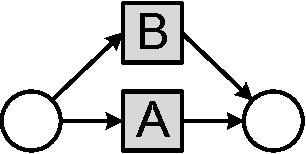
\includegraphics[width=0.3\textwidth]{uniqueness_2_d}
    \end{minipage}
    \begin{minipage}[b]{0.3\textwidth}
      \vspace{1em}
      \centering
      \begin{tabular}{|c|c|c|c|c|} \hline
        $\rightarrow$ & $\bm{S}$ & $A$ & $B$ & $\bm{E}$\\ \hline
        $\bm{S}$ & $\overset{\text{\tiny{N}}}{\rightarrow}$ & $\overset{\text{\tiny{DS}}}{\rightarrow}$ & $\overset{\text{\tiny{DS}}}{\rightarrow}$ & $\overset{\text{\tiny{IA}}}{\rightarrow}$\\ \hline
        $A$ & $\overset{\text{\tiny{N}}}{\rightarrow}$ & $\overset{\text{\tiny{N}}}{\rightarrow}$ & $\overset{\text{\tiny{N}}}{\rightarrow}$ & $\overset{\text{\tiny{DA}}}{\rightarrow}$\\ \hline
        $B$ & $\overset{\text{\tiny{N}}}{\rightarrow}$ & $\overset{\text{\tiny{N}}}{\rightarrow}$ & $\overset{\text{\tiny{N}}}{\rightarrow}$ & $\overset{\text{\tiny{DA}}}{\rightarrow}$\\ \hline
        $\bm{E}$ & $\overset{\text{\tiny{N}}}{\rightarrow}$ & $\overset{\text{\tiny{N}}}{\rightarrow}$ & $\overset{\text{\tiny{N}}}{\rightarrow}$ & $\overset{\text{\tiny{N}}}{\rightarrow}$\\ \hline
      \end{tabular}
    \end{minipage}
    \begin{minipage}[b]{0.3\textwidth}
      \vspace{1em}
      \centering
      \begin{tabular}{|c|c|c|c|c|} \hline
        $\leftarrow$ & $\bm{S}$ & $A$ & $B$ & $\bm{E}$\\ \hline
        $\bm{S}$ & $\overset{\text{\tiny{N}}}{\leftarrow}$ & $\overset{\text{\tiny{N}}}{\leftarrow}$ & $\overset{\text{\tiny{N}}}{\leftarrow}$ & $\overset{\text{\tiny{N}}}{\leftarrow}$\\ \hline
        $A$ & $\overset{\text{\tiny{DA}}}{\leftarrow}$ & $\overset{\text{\tiny{N}}}{\leftarrow}$ & $\overset{\text{\tiny{N}}}{\leftarrow}$ & $\overset{\text{\tiny{N}}}{\leftarrow}$\\ \hline
        $B$ & $\overset{\text{\tiny{DA}}}{\leftarrow}$ & $\overset{\text{\tiny{N}}}{\leftarrow}$ & $\overset{\text{\tiny{N}}}{\leftarrow}$ & $\overset{\text{\tiny{N}}}{\leftarrow}$\\ \hline
        $\bm{E}$ & $\overset{\text{\tiny{IA}}}{\leftarrow}$ & $\overset{\text{\tiny{DS}}}{\leftarrow}$ & $\overset{\text{\tiny{DS}}}{\leftarrow}$ & $\overset{\text{\tiny{N}}}{\leftarrow}$\\ \hline
      \end{tabular}
    \end{minipage}
    \begin{minipage}[b]{0.3\textwidth}
      \vspace{1em}
      \centering
      \begin{tabular}{|c|c|c|c|c|} \hline
        $\parallel$ & $\bm{S}$ & $A$ & $B$ & $\bm{E}$\\ \hline
        $\bm{S}$ & $\nparallel$ & $\nparallel$ & $\nparallel$ & $\nparallel$\\ \hline
        $A$ & $\nparallel$ & $\nparallel$ & $\nparallel$ & $\nparallel$\\ \hline
        $B$ & $\nparallel$ & $\nparallel$ & $\nparallel$ & $\nparallel$\\ \hline
        $\bm{E}$ & $\nparallel$ & $\nparallel$ & $\nparallel$ & $\nparallel$\\ \hline
      \end{tabular}
    \end{minipage}
    \caption{在\subref{fig:uniqueness_2_a}中增加一个可见变迁$B$,与$A$同处互斥结构}
    \label{fig:uniqueness_2_d}
  \end{subfigure}
  \vspace{6pt}
  \caption{向原始模型增加一个可见变迁}
\end{figure}

\begin{figure}[htbp]\ContinuedFloat
  \centering
  \begin{subfigure}{1\textwidth}
    \centering
    \begin{minipage}[b]{1\textwidth}
      \centering
      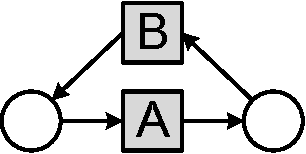
\includegraphics[width=0.3\textwidth]{uniqueness_2_e}
    \end{minipage}
    \begin{minipage}[b]{0.3\textwidth}
      \vspace{1em}
      \centering
      \begin{tabular}{|c|c|c|c|c|} \hline
        $\rightarrow$ & $\bm{S}$ & $A$ & $B$ & $\bm{E}$\\ \hline
        $\bm{S}$ & $\overset{\text{\tiny{N}}}{\rightarrow}$ & $\overset{\text{\tiny{DA}}}{\rightarrow}$ & $\overset{\text{\tiny{IS}}}{\rightarrow}$ & $\overset{\text{\tiny{IA}}}{\rightarrow}$\\ \hline
        $A$ & $\overset{\text{\tiny{N}}}{\rightarrow}$ & $\overset{\text{\tiny{IS}}}{\rightarrow}$ & $\overset{\text{\tiny{DS}}}{\rightarrow}$ & $\overset{\text{\tiny{DS}}}{\rightarrow}$\\ \hline
        $B$ & $\overset{\text{\tiny{N}}}{\rightarrow}$ & $\overset{\text{\tiny{DA}}}{\rightarrow}$ & $\overset{\text{\tiny{IS}}}{\rightarrow}$ & $\overset{\text{\tiny{IS}}}{\rightarrow}$\\ \hline
        $\bm{E}$ & $\overset{\text{\tiny{N}}}{\rightarrow}$ & $\overset{\text{\tiny{N}}}{\rightarrow}$ & $\overset{\text{\tiny{N}}}{\rightarrow}$ & $\overset{\text{\tiny{N}}}{\rightarrow}$\\ \hline
      \end{tabular}
    \end{minipage}
    \begin{minipage}[b]{0.3\textwidth}
      \vspace{1em}
      \centering
      \begin{tabular}{|c|c|c|c|c|} \hline
        $\leftarrow$ & $\bm{S}$ & $A$ & $B$ & $\bm{E}$\\ \hline
        $\bm{S}$ & $\overset{\text{\tiny{N}}}{\leftarrow}$ & $\overset{\text{\tiny{N}}}{\leftarrow}$ & $\overset{\text{\tiny{N}}}{\leftarrow}$ & $\overset{\text{\tiny{N}}}{\leftarrow}$\\ \hline
        $A$ & $\overset{\text{\tiny{DS}}}{\leftarrow}$ & $\overset{\text{\tiny{IS}}}{\leftarrow}$ & $\overset{\text{\tiny{DS}}}{\leftarrow}$ & $\overset{\text{\tiny{N}}}{\leftarrow}$\\ \hline
        $B$ & $\overset{\text{\tiny{IS}}}{\leftarrow}$ & $\overset{\text{\tiny{DA}}}{\leftarrow}$ & $\overset{\text{\tiny{IS}}}{\leftarrow}$ & $\overset{\text{\tiny{N}}}{\leftarrow}$\\ \hline
        $\bm{E}$ & $\overset{\text{\tiny{IA}}}{\leftarrow}$ & $\overset{\text{\tiny{DA}}}{\leftarrow}$ & $\overset{\text{\tiny{IS}}}{\leftarrow}$ & $\overset{\text{\tiny{N}}}{\leftarrow}$\\ \hline
      \end{tabular}
    \end{minipage}
    \begin{minipage}[b]{0.3\textwidth}
      \vspace{1em}
      \centering
      \begin{tabular}{|c|c|c|c|c|} \hline
        $\parallel$ & $\bm{S}$ & $A$ & $B$ & $\bm{E}$\\ \hline
        $\bm{S}$ & $\nparallel$ & $\nparallel$ & $\nparallel$ & $\nparallel$\\ \hline
        $A$ & $\nparallel$ & $\nparallel$ & $\nparallel$ & $\nparallel$\\ \hline
        $B$ & $\nparallel$ & $\nparallel$ & $\nparallel$ & $\nparallel$\\ \hline
        $\bm{E}$ & $\nparallel$ & $\nparallel$ & $\nparallel$ & $\nparallel$\\ \hline
      \end{tabular}
    \end{minipage}
    \caption{在\subref{fig:uniqueness_2_a}中增加一个可见变迁$B$,与$A$同处循环结构}
    \label{fig:uniqueness_2_e}
  \end{subfigure}

  \begin{subfigure}{1\textwidth}
    \vspace{1em}
    \centering
    \begin{minipage}[b]{1\textwidth}
      \centering
      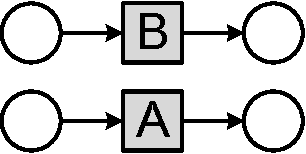
\includegraphics[width=0.3\textwidth]{uniqueness_2_f}
    \end{minipage}
    \begin{minipage}[b]{0.3\textwidth}
      \vspace{1em}
      \centering
      \begin{tabular}{|c|c|c|c|c|} \hline
        $\rightarrow$ & $\bm{S}$ & $A$ & $B$ & $\bm{E}$\\ \hline
        $\bm{S}$ & $\overset{\text{\tiny{N}}}{\rightarrow}$ & $\overset{\text{\tiny{DA}}}{\rightarrow}$ & $\overset{\text{\tiny{DA}}}{\rightarrow}$ & $\overset{\text{\tiny{IA}}}{\rightarrow}$\\ \hline
        $A$ & $\overset{\text{\tiny{N}}}{\rightarrow}$ & $\overset{\text{\tiny{N}}}{\rightarrow}$ & $\overset{\text{\tiny{N}}}{\rightarrow}$ & $\overset{\text{\tiny{DA}}}{\rightarrow}$\\ \hline
        $B$ & $\overset{\text{\tiny{N}}}{\rightarrow}$ & $\overset{\text{\tiny{N}}}{\rightarrow}$ & $\overset{\text{\tiny{N}}}{\rightarrow}$ & $\overset{\text{\tiny{DA}}}{\rightarrow}$\\ \hline
        $\bm{E}$ & $\overset{\text{\tiny{N}}}{\rightarrow}$ & $\overset{\text{\tiny{N}}}{\rightarrow}$ & $\overset{\text{\tiny{N}}}{\rightarrow}$ & $\overset{\text{\tiny{N}}}{\rightarrow}$\\ \hline
      \end{tabular}
    \end{minipage}
    \begin{minipage}[b]{0.3\textwidth}
      \vspace{1em}
      \centering
      \begin{tabular}{|c|c|c|c|c|} \hline
        $\leftarrow$ & $\bm{S}$ & $A$ & $B$ & $\bm{E}$\\ \hline
        $\bm{S}$ & $\overset{\text{\tiny{N}}}{\leftarrow}$ & $\overset{\text{\tiny{N}}}{\leftarrow}$ & $\overset{\text{\tiny{N}}}{\leftarrow}$ & $\overset{\text{\tiny{N}}}{\leftarrow}$\\ \hline
        $A$ & $\overset{\text{\tiny{DA}}}{\leftarrow}$ & $\overset{\text{\tiny{N}}}{\leftarrow}$ & $\overset{\text{\tiny{N}}}{\leftarrow}$ & $\overset{\text{\tiny{N}}}{\leftarrow}$\\ \hline
        $B$ & $\overset{\text{\tiny{DA}}}{\leftarrow}$ & $\overset{\text{\tiny{N}}}{\leftarrow}$ & $\overset{\text{\tiny{N}}}{\leftarrow}$ & $\overset{\text{\tiny{N}}}{\leftarrow}$\\ \hline
        $\bm{E}$ & $\overset{\text{\tiny{IA}}}{\leftarrow}$ & $\overset{\text{\tiny{DA}}}{\leftarrow}$ & $\overset{\text{\tiny{DA}}}{\leftarrow}$ & $\overset{\text{\tiny{N}}}{\leftarrow}$\\ \hline
      \end{tabular}
    \end{minipage}
    \begin{minipage}[b]{0.3\textwidth}
      \vspace{1em}
      \centering
      \begin{tabular}{|c|c|c|c|c|} \hline
        $\parallel$ & $\bm{S}$ & $A$ & $B$ & $\bm{E}$\\ \hline
        $\bm{S}$ & $\nparallel$ & $\nparallel$ & $\nparallel$ & $\nparallel$\\ \hline
        $A$ & $\nparallel$ & $\nparallel$ & $\Updownarrow$ & $\nparallel$\\ \hline
        $B$ & $\nparallel$ & $\Updownarrow$ & $\nparallel$ & $\nparallel$\\ \hline
        $\bm{E}$ & $\nparallel$ & $\nparallel$ & $\nparallel$ & $\nparallel$\\ \hline
      \end{tabular}
    \end{minipage}
    \caption{在\subref{fig:uniqueness_2_a}中增加一个可见变迁$B$,与$A$同处并行结构}
    \label{fig:uniqueness_2_f}
  \end{subfigure}
%     \caption{向原始模型增加一个可见变迁}
% \end{figure}

% \begin{figure}[htbp]\ContinuedFloat
%   \centering
  \vspace{6pt}
  \caption{向原始模型增加一个可见变迁(续)}
  \label{fig:uniqueness_2}
\end{figure}

\begin{figure}[htbp]
  \centering

  \begin{subfigure}{1\textwidth}
    \centering
    \begin{minipage}[b]{1\textwidth}
      \centering
      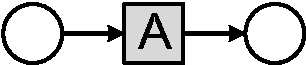
\includegraphics[width=0.3\textwidth]{uniqueness_3_a}
    \end{minipage}
    \begin{minipage}[b]{0.3\textwidth}
      \vspace{1em}
      \centering
      \begin{tabular}{|c|c|c|c|} \hline
        $\rightarrow$ & $\bm{S}$ & $A$ & $\bm{E}$\\ \hline
        $\bm{S}$ & $\overset{\text{\tiny{N}}}{\rightarrow}$ & $\overset{\text{\tiny{DA}}}{\rightarrow}$ & $\overset{\text{\tiny{IA}}}{\rightarrow}$\\ \hline
        $A$ & $\overset{\text{\tiny{N}}}{\rightarrow}$ & $\overset{\text{\tiny{N}}}{\rightarrow}$ & $\overset{\text{\tiny{DA}}}{\rightarrow}$\\ \hline
        $\bm{E}$ & $\overset{\text{\tiny{N}}}{\rightarrow}$ & $\overset{\text{\tiny{N}}}{\rightarrow}$ & $\overset{\text{\tiny{N}}}{\rightarrow}$\\ \hline
      \end{tabular}
    \end{minipage}
    \begin{minipage}[b]{0.3\textwidth}
      \vspace{1em}
      \centering
      \begin{tabular}{|c|c|c|c|} \hline
        $\leftarrow$ & $\bm{S}$ & $A$ & $\bm{E}$\\ \hline
        $\bm{S}$ & $\overset{\text{\tiny{N}}}{\leftarrow}$ & $\overset{\text{\tiny{N}}}{\leftarrow}$ & $\overset{\text{\tiny{N}}}{\leftarrow}$\\ \hline
        $A$ & $\overset{\text{\tiny{DA}}}{\leftarrow}$ & $\overset{\text{\tiny{N}}}{\leftarrow}$ & $\overset{\text{\tiny{N}}}{\leftarrow}$\\ \hline
        $\bm{E}$ & $\overset{\text{\tiny{IA}}}{\leftarrow}$ & $\overset{\text{\tiny{DA}}}{\leftarrow}$ & $\overset{\text{\tiny{N}}}{\leftarrow}$\\ \hline
      \end{tabular}
    \end{minipage}
    \begin{minipage}[b]{0.3\textwidth}
      \vspace{1em}
      \centering
      \begin{tabular}{|c|c|c|c|} \hline
        $\parallel$ & $\bm{S}$ & $A$ & $\bm{E}$\\ \hline
        $\bm{S}$ & $\nparallel$ & $\nparallel$ & $\nparallel$\\ \hline
        $A$ & $\nparallel$ & $\nparallel$ & $\nparallel$\\ \hline
        $\bm{E}$ & $\nparallel$ & $\nparallel$ & $\nparallel$\\ \hline
      \end{tabular}
    \end{minipage}
    \caption{原始部分模型,只含有可见变迁$A$}
    \label{fig:uniqueness_3_a}
  \end{subfigure}
  \vspace{6pt}
  \caption{向原始模型增加一个不可见变迁}
\end{figure}

\begin{figure}[htbp]\ContinuedFloat
  \centering
  \begin{subfigure}{1\textwidth}
    \centering
    \begin{minipage}[b]{1\textwidth}
      \centering
      
\includegraphics[width=0.11\textwidth]{uniqueness_3_b}
    \end{minipage}
    \begin{minipage}[b]{0.3\textwidth}
      \vspace{1em}
      \centering
      \begin{tabular}{|c|c|c|c|} \hline
        $\rightarrow$ & $\bm{S}$ & $A$ & $\bm{E}$\\ \hline
        $\bm{S}$ & $\overset{\text{\tiny{N}}}{\rightarrow}$ & $\overset{\text{\tiny{DS}}}{\rightarrow}$ & $\overset{\text{\tiny{DA}}}{\rightarrow}$\\ \hline
        $A$ & $\overset{\text{\tiny{N}}}{\rightarrow}$ & $\overset{\text{\tiny{DS}}}{\rightarrow}$ & $\overset{\text{\tiny{DS}}}{\rightarrow}$\\ \hline
        $\bm{E}$ & $\overset{\text{\tiny{N}}}{\rightarrow}$ & $\overset{\text{\tiny{N}}}{\rightarrow}$ & $\overset{\text{\tiny{N}}}{\rightarrow}$\\ \hline
      \end{tabular}
    \end{minipage}
    \begin{minipage}[b]{0.3\textwidth}
      \vspace{1em}
      \centering
      \begin{tabular}{|c|c|c|c|} \hline
        $\leftarrow$ & $\bm{S}$ & $A$ & $\bm{E}$\\ \hline
        $\bm{S}$ & $\overset{\text{\tiny{N}}}{\leftarrow}$ & $\overset{\text{\tiny{N}}}{\leftarrow}$ & $\overset{\text{\tiny{N}}}{\leftarrow}$\\ \hline
        $A$ & $\overset{\text{\tiny{DA}}}{\leftarrow}$ & $\overset{\text{\tiny{DS}}}{\leftarrow}$ & $\overset{\text{\tiny{N}}}{\leftarrow}$\\ \hline
        $\bm{E}$ & $\overset{\text{\tiny{DA}}}{\leftarrow}$ & $\overset{\text{\tiny{DS}}}{\leftarrow}$ & $\overset{\text{\tiny{N}}}{\leftarrow}$\\ \hline
      \end{tabular}
    \end{minipage}
    \begin{minipage}[b]{0.3\textwidth}
      \vspace{1em}
      \centering
      \begin{tabular}{|c|c|c|c|} \hline
        $\parallel$ & $\bm{S}$ & $A$ & $\bm{E}$\\ \hline
        $\bm{S}$ & $\nparallel$ & $\nparallel$ & $\nparallel$\\ \hline
        $A$ & $\nparallel$ & $\nparallel$ & $\nparallel$\\ \hline
        $\bm{E}$ & $\nparallel$ & $\nparallel$ & $\nparallel$\\ \hline
      \end{tabular}
    \end{minipage}
    \caption{将\subref{fig:uniqueness_3_a}中的两个库所合并成一个库所}
    \label{fig:uniqueness_3_b}
  \end{subfigure}

  \begin{subfigure}{1\textwidth}
    \vspace{1em}
    \centering
    \begin{minipage}[b]{1\textwidth}
      \centering
      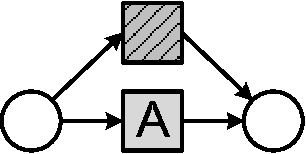
\includegraphics[width=0.3\textwidth]{uniqueness_3_c}
    \end{minipage}
    \begin{minipage}[b]{0.3\textwidth}
      \vspace{1em}
      \centering
      \begin{tabular}{|c|c|c|c|} \hline
        $\rightarrow$ & $\bm{S}$ & $A$ & $\bm{E}$\\ \hline
        $\bm{S}$ & $\overset{\text{\tiny{N}}}{\rightarrow}$ & $\overset{\text{\tiny{DS}}}{\rightarrow}$ & $\overset{\text{\tiny{DA}}}{\rightarrow}$\\ \hline
        $A$ & $\overset{\text{\tiny{N}}}{\rightarrow}$ & $\overset{\text{\tiny{N}}}{\rightarrow}$ & $\overset{\text{\tiny{DA}}}{\rightarrow}$\\ \hline
        $\bm{E}$ & $\overset{\text{\tiny{N}}}{\rightarrow}$ & $\overset{\text{\tiny{N}}}{\rightarrow}$ & $\overset{\text{\tiny{N}}}{\rightarrow}$\\ \hline
      \end{tabular}
    \end{minipage}
    \begin{minipage}[b]{0.3\textwidth}
      \vspace{1em}
      \centering
      \begin{tabular}{|c|c|c|c|} \hline
        $\leftarrow$ & $\bm{S}$ & $A$ & $\bm{E}$\\ \hline
        $\bm{S}$ & $\overset{\text{\tiny{N}}}{\leftarrow}$ & $\overset{\text{\tiny{N}}}{\leftarrow}$ & $\overset{\text{\tiny{N}}}{\leftarrow}$\\ \hline
        $A$ & $\overset{\text{\tiny{DA}}}{\leftarrow}$ & $\overset{\text{\tiny{N}}}{\leftarrow}$ & $\overset{\text{\tiny{N}}}{\leftarrow}$\\ \hline
        $\bm{E}$ & $\overset{\text{\tiny{DA}}}{\leftarrow}$ & $\overset{\text{\tiny{DS}}}{\leftarrow}$ & $\overset{\text{\tiny{N}}}{\leftarrow}$\\ \hline
      \end{tabular}
    \end{minipage}
    \begin{minipage}[b]{0.3\textwidth}
      \vspace{1em}
      \centering
      \begin{tabular}{|c|c|c|c|} \hline
        $\parallel$ & $\bm{S}$ & $A$ & $\bm{E}$\\ \hline
        $\bm{S}$ & $\nparallel$ & $\nparallel$ & $\nparallel$\\ \hline
        $A$ & $\nparallel$ & $\nparallel$ & $\nparallel$\\ \hline
        $\bm{E}$ & $\nparallel$ & $\nparallel$ & $\nparallel$\\ \hline
      \end{tabular}
    \end{minipage}
    \caption{在\subref{fig:uniqueness_3_a}中增加一个不可见变迁,与$A$同处互斥结构}
    \label{fig:uniqueness_3_c}
  \end{subfigure}

  \begin{subfigure}{1\textwidth}
    \vspace{1em}
    \centering
    \begin{minipage}[b]{1\textwidth}
      \centering
      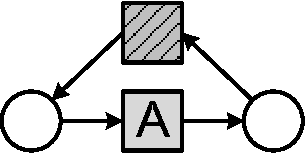
\includegraphics[width=0.3\textwidth]{uniqueness_3_d}
    \end{minipage}
    \begin{minipage}[b]{0.3\textwidth}
      \vspace{1em}
      \centering
      \begin{tabular}{|c|c|c|c|} \hline
        $\rightarrow$ & $\bm{S}$ & $A$ & $\bm{E}$\\ \hline
        $\bm{S}$ & $\overset{\text{\tiny{N}}}{\rightarrow}$ & $\overset{\text{\tiny{DA}}}{\rightarrow}$ & $\overset{\text{\tiny{IA}}}{\rightarrow}$\\ \hline
        $A$ & $\overset{\text{\tiny{N}}}{\rightarrow}$ & $\overset{\text{\tiny{DS}}}{\rightarrow}$ & $\overset{\text{\tiny{DS}}}{\rightarrow}$\\ \hline
        $\bm{E}$ & $\overset{\text{\tiny{N}}}{\rightarrow}$ & $\overset{\text{\tiny{N}}}{\rightarrow}$ & $\overset{\text{\tiny{N}}}{\rightarrow}$\\ \hline
      \end{tabular}
    \end{minipage}
    \begin{minipage}[b]{0.3\textwidth}
      \vspace{1em}
      \centering
      \begin{tabular}{|c|c|c|c|} \hline
        $\leftarrow$ & $\bm{S}$ & $A$ & $\bm{E}$\\ \hline
        $\bm{S}$ & $\overset{\text{\tiny{N}}}{\leftarrow}$ & $\overset{\text{\tiny{N}}}{\leftarrow}$ & $\overset{\text{\tiny{N}}}{\leftarrow}$\\ \hline
        $A$ & $\overset{\text{\tiny{DS}}}{\leftarrow}$ & $\overset{\text{\tiny{DS}}}{\leftarrow}$ & $\overset{\text{\tiny{N}}}{\leftarrow}$\\ \hline
        $\bm{E}$ & $\overset{\text{\tiny{IA}}}{\leftarrow}$ & $\overset{\text{\tiny{DA}}}{\leftarrow}$ & $\overset{\text{\tiny{N}}}{\leftarrow}$\\ \hline
      \end{tabular}
    \end{minipage}
    \begin{minipage}[b]{0.3\textwidth}
      \vspace{1em}
      \centering
      \begin{tabular}{|c|c|c|c|} \hline
        $\parallel$ & $\bm{S}$ & $A$ & $\bm{E}$\\ \hline
        $\bm{S}$ & $\nparallel$ & $\nparallel$ & $\nparallel$\\ \hline
        $A$ & $\nparallel$ & $\nparallel$ & $\nparallel$\\ \hline
        $\bm{E}$ & $\nparallel$ & $\nparallel$ & $\nparallel$\\ \hline
      \end{tabular}
    \end{minipage}
    \caption{在\subref{fig:uniqueness_3_a}中增加一个不可见变迁,与$A$同处循环结构}
    \label{fig:uniqueness_3_d}
  \end{subfigure}
  \vspace{6pt}
  \caption{向原始模型增加一个不可见变迁(续)}
\end{figure}

\begin{figure}[htbp]\ContinuedFloat
  \centering
  \begin{subfigure}{1\textwidth}
    \centering
    \begin{minipage}[b]{1\textwidth}
      \centering
      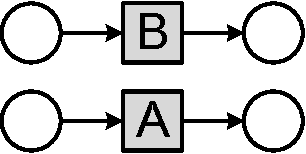
\includegraphics[width=0.3\textwidth]{uniqueness_3_e}
    \end{minipage}
    \begin{minipage}[b]{0.3\textwidth}
      \vspace{1em}
      \centering
      \begin{tabular}{|c|c|c|c|c|} \hline
        $\rightarrow$ & $\bm{S}$ & $A$ & $B$ & $\bm{E}$\\ \hline
        $\bm{S}$ & $\overset{\text{\tiny{N}}}{\rightarrow}$ & $\overset{\text{\tiny{DA}}}{\rightarrow}$ & $\overset{\text{\tiny{DA}}}{\rightarrow}$ & $\overset{\text{\tiny{IA}}}{\rightarrow}$\\ \hline
        $A$ & $\overset{\text{\tiny{N}}}{\rightarrow}$ & $\overset{\text{\tiny{N}}}{\rightarrow}$ & $\overset{\text{\tiny{N}}}{\rightarrow}$ & $\overset{\text{\tiny{DA}}}{\rightarrow}$\\ \hline
        $B$ & $\overset{\text{\tiny{N}}}{\rightarrow}$ & $\overset{\text{\tiny{N}}}{\rightarrow}$ & $\overset{\text{\tiny{N}}}{\rightarrow}$ & $\overset{\text{\tiny{DA}}}{\rightarrow}$\\ \hline
        $\bm{E}$ & $\overset{\text{\tiny{N}}}{\rightarrow}$ & $\overset{\text{\tiny{N}}}{\rightarrow}$ & $\overset{\text{\tiny{N}}}{\rightarrow}$ & $\overset{\text{\tiny{N}}}{\rightarrow}$\\ \hline
      \end{tabular}
    \end{minipage}
    \begin{minipage}[b]{0.3\textwidth}
      \vspace{1em}
      \centering
      \begin{tabular}{|c|c|c|c|c|} \hline
        $\leftarrow$ & $\bm{S}$ & $A$ & $B$ & $\bm{E}$\\ \hline
        $\bm{S}$ & $\overset{\text{\tiny{N}}}{\leftarrow}$ & $\overset{\text{\tiny{N}}}{\leftarrow}$ & $\overset{\text{\tiny{N}}}{\leftarrow}$ & $\overset{\text{\tiny{N}}}{\leftarrow}$\\ \hline
        $A$ & $\overset{\text{\tiny{DA}}}{\leftarrow}$ & $\overset{\text{\tiny{N}}}{\leftarrow}$ & $\overset{\text{\tiny{N}}}{\leftarrow}$ & $\overset{\text{\tiny{N}}}{\leftarrow}$\\ \hline
        $B$ & $\overset{\text{\tiny{DA}}}{\leftarrow}$ & $\overset{\text{\tiny{N}}}{\leftarrow}$ & $\overset{\text{\tiny{N}}}{\leftarrow}$ & $\overset{\text{\tiny{N}}}{\leftarrow}$\\ \hline
        $\bm{E}$ & $\overset{\text{\tiny{IA}}}{\leftarrow}$ & $\overset{\text{\tiny{DA}}}{\leftarrow}$ & $\overset{\text{\tiny{DA}}}{\leftarrow}$ & $\overset{\text{\tiny{N}}}{\leftarrow}$\\ \hline
      \end{tabular}
    \end{minipage}
    \begin{minipage}[b]{0.3\textwidth}
      \vspace{1em}
      \centering
      \begin{tabular}{|c|c|c|c|c|} \hline
        $\parallel$ & $\bm{S}$ & $A$ & $B$ & $\bm{E}$\\ \hline
        $\bm{S}$ & $\nparallel$ & $\nparallel$ & $\nparallel$ & $\nparallel$\\ \hline
        $A$ & $\nparallel$ & $\nparallel$ & $\Updownarrow$ & $\nparallel$\\ \hline
        $B$ & $\nparallel$ & $\Updownarrow$ & $\nparallel$ & $\nparallel$\\ \hline
        $\bm{E}$ & $\nparallel$ & $\nparallel$ & $\nparallel$ & $\nparallel$\\ \hline
      \end{tabular}
    \end{minipage}
    \caption{另一个原始部分模型,含有两个处于并行结构的变迁$A$和变迁$B$}
    \label{fig:uniqueness_3_e}
  \end{subfigure}

  \begin{subfigure}{1\textwidth}
    \vspace{1em}
    \centering
    \begin{minipage}[b]{1\textwidth}
      \centering
      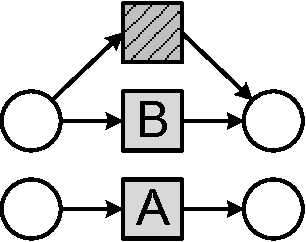
\includegraphics[width=0.3\textwidth]{uniqueness_3_f}
    \end{minipage}
    \begin{minipage}[b]{0.3\textwidth}
      \vspace{1em}
      \centering
      \begin{tabular}{|c|c|c|c|c|} \hline
        $\rightarrow$ & $\bm{S}$ & $A$ & $B$ & $\bm{E}$\\ \hline
        $\bm{S}$ & $\overset{\text{\tiny{N}}}{\rightarrow}$ & $\overset{\text{\tiny{DA}}}{\rightarrow}$ & $\overset{\text{\tiny{DS}}}{\rightarrow}$ & $\overset{\text{\tiny{IA}}}{\rightarrow}$\\ \hline
        $A$ & $\overset{\text{\tiny{N}}}{\rightarrow}$ & $\overset{\text{\tiny{N}}}{\rightarrow}$ & $\overset{\text{\tiny{N}}}{\rightarrow}$ & $\overset{\text{\tiny{DA}}}{\rightarrow}$\\ \hline
        $B$ & $\overset{\text{\tiny{N}}}{\rightarrow}$ & $\overset{\text{\tiny{N}}}{\rightarrow}$ & $\overset{\text{\tiny{N}}}{\rightarrow}$ & $\overset{\text{\tiny{DA}}}{\rightarrow}$\\ \hline
        $\bm{E}$ & $\overset{\text{\tiny{N}}}{\rightarrow}$ & $\overset{\text{\tiny{N}}}{\rightarrow}$ & $\overset{\text{\tiny{N}}}{\rightarrow}$ & $\overset{\text{\tiny{N}}}{\rightarrow}$\\ \hline
      \end{tabular}
    \end{minipage}
    \begin{minipage}[b]{0.3\textwidth}
      \vspace{1em}
      \centering
      \begin{tabular}{|c|c|c|c|c|} \hline
        $\leftarrow$ & $\bm{S}$ & $A$ & $B$ & $\bm{E}$\\ \hline
        $\bm{S}$ & $\overset{\text{\tiny{N}}}{\leftarrow}$ & $\overset{\text{\tiny{N}}}{\leftarrow}$ & $\overset{\text{\tiny{N}}}{\leftarrow}$ & $\overset{\text{\tiny{N}}}{\leftarrow}$\\ \hline
        $A$ & $\overset{\text{\tiny{DA}}}{\leftarrow}$ & $\overset{\text{\tiny{N}}}{\leftarrow}$ & $\overset{\text{\tiny{N}}}{\leftarrow}$ & $\overset{\text{\tiny{N}}}{\leftarrow}$\\ \hline
        $B$ & $\overset{\text{\tiny{DA}}}{\leftarrow}$ & $\overset{\text{\tiny{N}}}{\leftarrow}$ & $\overset{\text{\tiny{N}}}{\leftarrow}$ & $\overset{\text{\tiny{N}}}{\leftarrow}$\\ \hline
        $\bm{E}$ & $\overset{\text{\tiny{IA}}}{\leftarrow}$ & $\overset{\text{\tiny{DA}}}{\leftarrow}$ & $\overset{\text{\tiny{DS}}}{\leftarrow}$ & $\overset{\text{\tiny{N}}}{\leftarrow}$\\ \hline
      \end{tabular}
    \end{minipage}
    \begin{minipage}[b]{0.3\textwidth}
      \vspace{1em}
      \centering
      \begin{tabular}{|c|c|c|c|c|} \hline
        $\parallel$ & $\bm{S}$ & $A$ & $B$ & $\bm{E}$\\ \hline
        $\bm{S}$ & $\nparallel$ & $\nparallel$ & $\nparallel$ & $\nparallel$\\ \hline
        $A$ & $\nparallel$ & $\nparallel$ & $\Uparrow$ & $\nparallel$\\ \hline
        $B$ & $\nparallel$ & $\Updownarrow$ & $\nparallel$ & $\nparallel$\\ \hline
        $\bm{E}$ & $\nparallel$ & $\nparallel$ & $\nparallel$ & $\nparallel$\\ \hline
      \end{tabular}
    \end{minipage}
    \caption{在\subref{fig:uniqueness_3_e}中增加一个不可见变迁,与$B$同处互斥结构}
    \label{fig:uniqueness_3_f}
  \end{subfigure}

  \begin{subfigure}{1\textwidth}
    \vspace{1em}
    \centering
    \begin{minipage}[b]{1\textwidth}
      \centering
      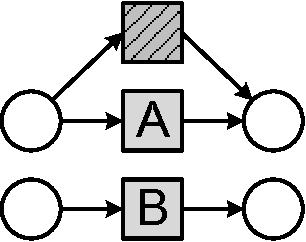
\includegraphics[width=0.3\textwidth]{uniqueness_3_g}
    \end{minipage}
    \begin{minipage}[b]{0.3\textwidth}
      \vspace{1em}
      \centering
      \begin{tabular}{|c|c|c|c|c|} \hline
        $\rightarrow$ & $\bm{S}$ & $A$ & $B$ & $\bm{E}$\\ \hline
        $\bm{S}$ & $\overset{\text{\tiny{N}}}{\rightarrow}$ & $\overset{\text{\tiny{DS}}}{\rightarrow}$ & $\overset{\text{\tiny{DA}}}{\rightarrow}$ & $\overset{\text{\tiny{IA}}}{\rightarrow}$\\ \hline
        $A$ & $\overset{\text{\tiny{N}}}{\rightarrow}$ & $\overset{\text{\tiny{N}}}{\rightarrow}$ & $\overset{\text{\tiny{N}}}{\rightarrow}$ & $\overset{\text{\tiny{DA}}}{\rightarrow}$\\ \hline
        $B$ & $\overset{\text{\tiny{N}}}{\rightarrow}$ & $\overset{\text{\tiny{N}}}{\rightarrow}$ & $\overset{\text{\tiny{N}}}{\rightarrow}$ & $\overset{\text{\tiny{DA}}}{\rightarrow}$\\ \hline
        $\bm{E}$ & $\overset{\text{\tiny{N}}}{\rightarrow}$ & $\overset{\text{\tiny{N}}}{\rightarrow}$ & $\overset{\text{\tiny{N}}}{\rightarrow}$ & $\overset{\text{\tiny{N}}}{\rightarrow}$\\ \hline
      \end{tabular}
    \end{minipage}
    \begin{minipage}[b]{0.3\textwidth}
      \vspace{1em}
      \centering
      \begin{tabular}{|c|c|c|c|c|} \hline
        $\leftarrow$ & $\bm{S}$ & $A$ & $B$ & $\bm{E}$\\ \hline
        $\bm{S}$ & $\overset{\text{\tiny{N}}}{\leftarrow}$ & $\overset{\text{\tiny{N}}}{\leftarrow}$ & $\overset{\text{\tiny{N}}}{\leftarrow}$ & $\overset{\text{\tiny{N}}}{\leftarrow}$\\ \hline
        $A$ & $\overset{\text{\tiny{DA}}}{\leftarrow}$ & $\overset{\text{\tiny{N}}}{\leftarrow}$ & $\overset{\text{\tiny{N}}}{\leftarrow}$ & $\overset{\text{\tiny{N}}}{\leftarrow}$\\ \hline
        $B$ & $\overset{\text{\tiny{DA}}}{\leftarrow}$ & $\overset{\text{\tiny{N}}}{\leftarrow}$ & $\overset{\text{\tiny{N}}}{\leftarrow}$ & $\overset{\text{\tiny{N}}}{\leftarrow}$\\ \hline
        $\bm{E}$ & $\overset{\text{\tiny{IA}}}{\leftarrow}$ & $\overset{\text{\tiny{DS}}}{\leftarrow}$ & $\overset{\text{\tiny{DA}}}{\leftarrow}$ & $\overset{\text{\tiny{N}}}{\leftarrow}$\\ \hline
      \end{tabular}
    \end{minipage}
    \begin{minipage}[b]{0.3\textwidth}
      \vspace{1em}
      \centering
      \begin{tabular}{|c|c|c|c|c|} \hline
        $\parallel$ & $\bm{S}$ & $A$ & $B$ & $\bm{E}$\\ \hline
        $\bm{S}$ & $\nparallel$ & $\nparallel$ & $\nparallel$ & $\nparallel$\\ \hline
        $A$ & $\nparallel$ & $\nparallel$ & $\Updownarrow$ & $\nparallel$\\ \hline
        $B$ & $\nparallel$ & $\Uparrow$ & $\nparallel$ & $\nparallel$\\ \hline
        $\bm{E}$ & $\nparallel$ & $\nparallel$ & $\nparallel$ & $\nparallel$\\ \hline
      \end{tabular}
    \end{minipage}
    \caption{在\subref{fig:uniqueness_3_e}中增加一个不可见变迁,与$A$同处互斥结构}
    \label{fig:uniqueness_3_g}
  \end{subfigure}
  \vspace{6pt}
  \caption{向原始模型增加一个不可见变迁(续)}
\end{figure}

\begin{figure}[htbp]\ContinuedFloat
  \centering
  \begin{subfigure}{1\textwidth}
    \centering
    \begin{minipage}[b]{1\textwidth}
      \centering
      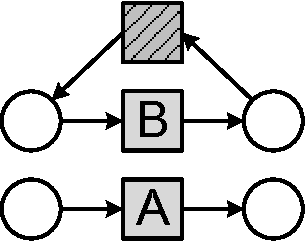
\includegraphics[width=0.3\textwidth]{uniqueness_3_h}
    \end{minipage}
    \begin{minipage}[b]{0.3\textwidth}
      \vspace{1em}
      \centering
      \begin{tabular}{|c|c|c|c|c|} \hline
        $\rightarrow$ & $\bm{S}$ & $A$ & $B$ & $\bm{E}$\\ \hline
        $\bm{S}$ & $\overset{\text{\tiny{N}}}{\rightarrow}$ & $\overset{\text{\tiny{DA}}}{\rightarrow}$ & $\overset{\text{\tiny{DA}}}{\rightarrow}$ & $\overset{\text{\tiny{IA}}}{\rightarrow}$\\ \hline
        $A$ & $\overset{\text{\tiny{N}}}{\rightarrow}$ & $\overset{\text{\tiny{N}}}{\rightarrow}$ & $\overset{\text{\tiny{N}}}{\rightarrow}$ & $\overset{\text{\tiny{DA}}}{\rightarrow}$\\ \hline
        $B$ & $\overset{\text{\tiny{N}}}{\rightarrow}$ & $\overset{\text{\tiny{N}}}{\rightarrow}$ & $\overset{\text{\tiny{DS}}}{\rightarrow}$ & $\overset{\text{\tiny{DS}}}{\rightarrow}$\\ \hline
        $\bm{E}$ & $\overset{\text{\tiny{N}}}{\rightarrow}$ & $\overset{\text{\tiny{N}}}{\rightarrow}$ & $\overset{\text{\tiny{N}}}{\rightarrow}$ & $\overset{\text{\tiny{N}}}{\rightarrow}$\\ \hline
      \end{tabular}
    \end{minipage}
    \begin{minipage}[b]{0.3\textwidth}
      \vspace{1em}
      \centering
      \begin{tabular}{|c|c|c|c|c|} \hline
        $\leftarrow$ & $\bm{S}$ & $A$ & $B$ & $\bm{E}$\\ \hline
        $\bm{S}$ & $\overset{\text{\tiny{N}}}{\leftarrow}$ & $\overset{\text{\tiny{N}}}{\leftarrow}$ & $\overset{\text{\tiny{N}}}{\leftarrow}$ & $\overset{\text{\tiny{N}}}{\leftarrow}$\\ \hline
        $A$ & $\overset{\text{\tiny{DA}}}{\leftarrow}$ & $\overset{\text{\tiny{N}}}{\leftarrow}$ & $\overset{\text{\tiny{N}}}{\leftarrow}$ & $\overset{\text{\tiny{N}}}{\leftarrow}$\\ \hline
        $B$ & $\overset{\text{\tiny{DS}}}{\leftarrow}$ & $\overset{\text{\tiny{N}}}{\leftarrow}$ & $\overset{\text{\tiny{DS}}}{\leftarrow}$ & $\overset{\text{\tiny{N}}}{\leftarrow}$\\ \hline
        $\bm{E}$ & $\overset{\text{\tiny{IA}}}{\leftarrow}$ & $\overset{\text{\tiny{DA}}}{\leftarrow}$ & $\overset{\text{\tiny{DA}}}{\leftarrow}$ & $\overset{\text{\tiny{N}}}{\leftarrow}$\\ \hline
      \end{tabular}
    \end{minipage}
    \begin{minipage}[b]{0.3\textwidth}
      \vspace{1em}
      \centering
      \begin{tabular}{|c|c|c|c|c|} \hline
        $\parallel$ & $\bm{S}$ & $A$ & $B$ & $\bm{E}$\\ \hline
        $\bm{S}$ & $\nparallel$ & $\nparallel$ & $\nparallel$ & $\nparallel$\\ \hline
        $A$ & $\nparallel$ & $\nparallel$ & $\Updownarrow$ & $\nparallel$\\ \hline
        $B$ & $\nparallel$ & $\Uparrow$ & $\nparallel$ & $\nparallel$\\ \hline
        $\bm{E}$ & $\nparallel$ & $\nparallel$ & $\nparallel$ & $\nparallel$\\ \hline
      \end{tabular}
    \end{minipage}
    \caption{在\subref{fig:uniqueness_3_e}中增加一个不可见变迁,与$B$同处循环结构}
    \label{fig:uniqueness_3_h}
  \end{subfigure}

  \begin{subfigure}{1\textwidth}
    \vspace{1em}
    \centering
    \begin{minipage}[b]{1\textwidth}
      \centering
      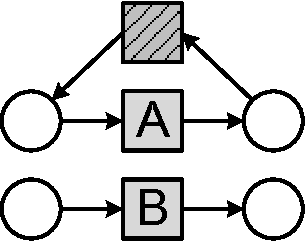
\includegraphics[width=0.3\textwidth]{uniqueness_3_i}
    \end{minipage}
    \begin{minipage}[b]{0.3\textwidth}
      \vspace{1em}
      \centering
      \begin{tabular}{|c|c|c|c|c|} \hline
        $\rightarrow$ & $\bm{S}$ & $A$ & $B$ & $\bm{E}$\\ \hline
        $\bm{S}$ & $\overset{\text{\tiny{N}}}{\rightarrow}$ & $\overset{\text{\tiny{DA}}}{\rightarrow}$ & $\overset{\text{\tiny{DA}}}{\rightarrow}$ & $\overset{\text{\tiny{IA}}}{\rightarrow}$\\ \hline
        $A$ & $\overset{\text{\tiny{N}}}{\rightarrow}$ & $\overset{\text{\tiny{DS}}}{\rightarrow}$ & $\overset{\text{\tiny{N}}}{\rightarrow}$ & $\overset{\text{\tiny{DS}}}{\rightarrow}$\\ \hline
        $B$ & $\overset{\text{\tiny{N}}}{\rightarrow}$ & $\overset{\text{\tiny{N}}}{\rightarrow}$ & $\overset{\text{\tiny{N}}}{\rightarrow}$ & $\overset{\text{\tiny{DA}}}{\rightarrow}$\\ \hline
        $\bm{E}$ & $\overset{\text{\tiny{N}}}{\rightarrow}$ & $\overset{\text{\tiny{N}}}{\rightarrow}$ & $\overset{\text{\tiny{N}}}{\rightarrow}$ & $\overset{\text{\tiny{N}}}{\rightarrow}$\\ \hline
      \end{tabular}
    \end{minipage}
    \begin{minipage}[b]{0.3\textwidth}
      \vspace{1em}
      \centering
      \begin{tabular}{|c|c|c|c|c|} \hline
        $\leftarrow$ & $\bm{S}$ & $A$ & $B$ & $\bm{E}$\\ \hline
        $\bm{S}$ & $\overset{\text{\tiny{N}}}{\leftarrow}$ & $\overset{\text{\tiny{N}}}{\leftarrow}$ & $\overset{\text{\tiny{N}}}{\leftarrow}$ & $\overset{\text{\tiny{N}}}{\leftarrow}$\\ \hline
        $A$ & $\overset{\text{\tiny{DS}}}{\leftarrow}$ & $\overset{\text{\tiny{DS}}}{\leftarrow}$ & $\overset{\text{\tiny{N}}}{\leftarrow}$ & $\overset{\text{\tiny{N}}}{\leftarrow}$\\ \hline
        $B$ & $\overset{\text{\tiny{DA}}}{\leftarrow}$ & $\overset{\text{\tiny{N}}}{\leftarrow}$ & $\overset{\text{\tiny{N}}}{\leftarrow}$ & $\overset{\text{\tiny{N}}}{\leftarrow}$\\ \hline
        $\bm{E}$ & $\overset{\text{\tiny{IA}}}{\leftarrow}$ & $\overset{\text{\tiny{DA}}}{\leftarrow}$ & $\overset{\text{\tiny{DA}}}{\leftarrow}$ & $\overset{\text{\tiny{N}}}{\leftarrow}$\\ \hline
      \end{tabular}
    \end{minipage}
    \begin{minipage}[b]{0.3\textwidth}
      \vspace{1em}
      \centering
      \begin{tabular}{|c|c|c|c|c|} \hline
        $\parallel$ & $\bm{S}$ & $A$ & $B$ & $\bm{E}$\\ \hline
        $\bm{S}$ & $\nparallel$ & $\nparallel$ & $\nparallel$ & $\nparallel$\\ \hline
        $A$ & $\nparallel$ & $\nparallel$ & $\Uparrow$ & $\nparallel$\\ \hline
        $B$ & $\nparallel$ & $\Updownarrow$ & $\nparallel$ & $\nparallel$\\ \hline
        $\bm{E}$ & $\nparallel$ & $\nparallel$ & $\nparallel$ & $\nparallel$\\ \hline
      \end{tabular}
    \end{minipage}
    \caption{在\subref{fig:uniqueness_3_e}中增加一个不可见变迁,与$A$同处循环结构}
    \label{fig:uniqueness_3_i}
  \end{subfigure}
  %     \caption{向原始模型增加一个不可见变迁}
% \end{figure}

% \begin{figure}[htbp]\ContinuedFloat
%   \centering
  \vspace{6pt}
  \caption{向原始模型增加一个不可见变迁(续)}
  \label{fig:uniqueness_3}
\end{figure}